%!TEX TS-program = xelatex
%!TEX encoding = UTF-8 Unicode
\documentclass[a4paper]{report}
%\usepackage[date=short,backend=biber]{apa}
\usepackage[hidelinks]{hyperref}
\usepackage{cite}
\usepackage[dutch]{babel}
\usepackage[a4paper, left=1in, right=1in, top=1in, bottom=.8in]{geometry}
\usepackage[utf8]{inputenc}
\usepackage{fancyhdr}
\usepackage{titlesec}
\usepackage{geometry}
\usepackage{graphicx}
\usepackage{etoolbox}
\usepackage{listings}
\usepackage{xcolor}
\usepackage{nameref}
\usepackage{tcolorbox}
\usepackage{textcomp}
\usepackage{helvet}
\usepackage{enumitem}
\usepackage{tabularx}
\usepackage{pgf-pie}  
\usepackage{float}
\usepackage{pgfplots}
% Styling
\pagestyle{fancy}
\patchcmd{\chapter}{\thispagestyle{plain}}{\thispagestyle{fancy}}{}{}

\fancyhf{}
\fancyhead[L]{ Team Fairphone }
\fancyhead[R]{Verantwoordingsdocument }
\fancyfoot[R]{\thepage}

\titleformat{\chapter}[hang]
{\normalfont\huge\bfseries}{\thechapter.}{10pt}{\huge}
\titlespacing{\chapter}{0pt}{-30pt}{20pt}

\setlength{\parindent}{0.2em}

\textwidth=400pt
\geometry{
    left=25mm
}

\renewcommand{\contentsname}{Inhoudsopgave}



\definecolor{codegreen}{rgb}{0,0.6,0}
\definecolor{codegray}{rgb}{0.5,0.5,0.5}
\definecolor{codepurple}{rgb}{0.58,0,0.82}
\definecolor{backcolour}{rgb}{0.95,0.95,0.92}

\lstdefinestyle{mystyle}{
    backgroundcolor=\color{backcolour},   
    commentstyle=\color{codegreen},
    keywordstyle=\color{magenta},
    numberstyle=\tiny\color{codegray},
    stringstyle=\color{codepurple},
    basicstyle=\ttfamily\footnotesize,
    breakatwhitespace=false,         
    breaklines=true,                 
    captionpos=b,                    
    keepspaces=true,                 
    numbers=left,                    
    numbersep=5pt,                  
    showspaces=false,                
    showstringspaces=false,
    showtabs=false,                  
    tabsize=2
}

\lstset{style=mystyle}

% Commands
\newcommand{\teambox}{
  \begin{tcolorbox}[hbox, colback=blue!5!white,colframe=blue!75!black,
    left=.1mm, right=.1mm, top=.1mm, bottom=.1mm, fontupper=\scriptsize\sffamily]
    Team Keuze
  \end{tcolorbox}
}

\newcommand{\personalbox}{
  \begin{tcolorbox}[hbox, colback=green!5!white,colframe=green!75!black,
    left=.1mm, right=.1mm, top=.1mm, bottom=.1mm, fontupper=\scriptsize\sffamily]
    Persoonlijke Keuze
  \end{tcolorbox}
}
\newcommand{\teamchoice}[1]{
  \section[ #1 ]{#1~\mbox{\raisebox{-2.5pt}{\teambox}}}
}

\newcommand{\personalchoice}[1]{
  \section[ #1 ]{#1~\mbox{\raisebox{-2.5pt}{\personalbox}}}
}

\newcommand{\timestamp}[1]{
  \mbox{\scriptsize \textbf{Datum:} #1} \smallbreak
}

% Document
\begin{document}


% Title Page
\begin{titlepage}
  \begin{center}
      \vspace*{.9cm}
      \Huge
      \textbf{ Verantwoordingsdocument }\\
      \vspace{0.2cm}
      \small Team FairPhone

      \normalsize


      \vspace{2cm}
      
\includegraphics[width=0.7\textwidth]{Images/fairphone.png}
      \vspace{2cm}
      \Large\\
      \textbf{In opdracht van}\\
      \large
      \textbf{Hogeschool Utrecht} \\
      
\includegraphics[width=0.2\textwidth]{Images/logouni.png}


      \vfill
    \end{center}
      \textbf{Student:} Vincent van Setten - 1734729 \\
      \textbf{Gilde:} TI Gilde, Groep D\\
      \textbf{Innovation Team:} Project FairPhone (499) \\
      \textbf{Datum:} \today \\
      \vspace{2cm}
\end{titlepage}



% ToC
\tableofcontents

\chapter{Versiebeheer}
\begin{table}[h]
    \centering
    \begin{tabular}{|c|c|c|p{5cm}|}
        \hline
        \textbf{Versie} & \textbf{Datum} & \textbf{Veranderingen}  \\
        \hline
        1.4    & 2023-09-25 & Meer details en visuals toegevoegd \\
        \hline
        1.3    & 2023-09-24 & Referenties toegevoegd \\
        \hline
        1.2    & 2023-09-22 & Hoofdstuk docker toegevoegd en keuzes uitgebreid \\
        \hline
        1.1    & 2023-09-14 & Introductie en timestamps toegevoegd\\
        \hline
        1.0    & 2023-09-10 & Eerste Versie \\
        \hline
    \end{tabular}
    \caption{Versiebeheer}
\end{table}


\chapter{Introductie}
Dit document heeft als doel het beschrijven en beredeneren van belangrijke gemaakte keuzes binnen het Innovation project. 
Hiermee kunnen stakeholders, toekomstige teams en projectleiders eenvoudig zien welke keuzes zijn gemaakt en waarom deze zijn gemaakt.
Daarmee hopen wij meer inzicht te bieden in het verloop van het project en waarom voor bepaalde dingen zijn gekozen. 
\vspace{1.5cm}

\begingroup
\let\clearpage\relax
\chapter{Projectbeschrijving}
Vanuit de Hogeschool Utrecht heeft ons team de opdracht gekregen om verder te werken aan een port van SailfishOS voor de Fairphone 4.
SailfishOS is een open-source besturingssysteem gemaakt door een bedrijf, Jolla, uit Finland. Standaard ondersteund SailfishOS geen Fairphone 4.
Vorig jaar heeft een ander team al een minimale port werkend gekregen, namelijk de basis functies van een operating system. Er missen daarentegen nog een aantal belangrijke functies.
\par \smallskip
Ons hoofddoel is het toevoegen van ondersteuning van android applicaties, zonder afhankelijk te zijn van Google en haar Google Play Services\texttrademark. 
Daarnaast gaan we ondersteuning toevoegen voor 4G, door Sailfish OS te updaten.
\endgroup

\chapter{Gemaakte Keuzes}
% \section{Persoonlijke Keuzes}
\personalchoice{IDE}
\subsubsection{Context}
\timestamp{2023-09-05}
Onze code gaan we schrijven met behulp van een IDE. Dit is een vrij arbitraire keuze, maar kan later in het project gevolgen hebben. 
Zo kan elke IDE zijn eigen methodes hebben voor het gebruik en delen van instellingen en linters. 
\par\smallskip
Er zijn een aantal grote IDE's die wij kunnen gebruiken voor dit project, welke wij hebben gekozen omdat we hier al eerder mee hebben gewerkt binnen de opleiding.
\begin{enumerate}
  \item \href{https://visualstudio.microsoft.com/}{Visual Studio} - Dit is een grote IDE met een breed scala aan features.
  \item \href{https://code.visualstudio.com/}{Visual Studio Code} - Dit is officieel geen echte IDE, maar kan helemaal samengesteld worden naar jouw eigen beeld.
  \item \href{https://codelite.org/}{CodeLite} - Dit is een bekend open-source IDE, gemaakt voor meerdere programmeertalen.
\end{enumerate}


\subsubsection{Keuze}
\timestamp{2023-09-05}
Voor de IDE heb ik gekozen voor Visual Studio Code. Officieel is het geen IDE, maar het wordt veelal wel gebruikt als een IDE. 
Door de vele extensies en aanpasbaarheid, kan deze editor volledig naar wens ingesteld worden. 
Het is een volledig persoonlijke keuze, maar iedereen in ons team heeft ook gekozen voor Visual Studio Code.
Dit kan in de toekomst werk schelen, doordat onze werkomgeving bij iedereen gelijk is.

\personalchoice{Laptop OS}
\subsubsection{Context}
\timestamp{2023-09-05}
Om aan Sailfish OS te kunnen werken in een ontwikkelomgeving moet er een keuze gemaakt worden op welk besturingssysteem de ontwikkelomgeving gaat draaien. 
Volgens de porting-guide van SailfishOS hebben we een 64-bit Linux kernel nodig om SailfishOS verder te ontwikkelen~\cite{sailfishportingguide}.
De mogelijkheden voor dit project zijn keuzes uit verschillende 64-bit Linux distributies. 

We hebben de volgende distributies vergeleken. De redenen voor de keuze van deze specifieke distributies staan hieronder verder toegelicht.
\begin{enumerate}
  \item \href{https://archlinux.org/}{Arch Linux}
  \item \href{https://ubuntu.com/}{Ubuntu}
  \item \href{https://www.debian.org/}{Debian}
  \item \href{https://manjaro.org/}{Manjaro}
\end{enumerate}


\subsubsection{Keuze}
\timestamp{2023-09-05}
Als team hebben we gekozen om Ubuntu te gebruiken als besturingssysteem voor onze laptops. 
Dit hebben we gedaan om de volgende twee redenen.
\begin{enumerate}
  \item Het voorgaande team gebruikte ook Linux en gebruikte dit voor de ontwikkelomgeving~\cite{fairphonegithub}
  \item De root-omgeving van SailfishOS is gebaseerd op Ubuntu (20.04 LTS)~\cite{sailfishportingguide}.
\end{enumerate}

Persoonlijk heb ik er voor gekozen om af te wijken van de team keuze, omdat ik denk dat ik efficiënter kan werken met een ander besturingssysteem.
Mijn team ging hier mee akkoord. Ik zal de specifieke redenen hieronder toelichten.
\par\smallskip
Ik heb sterke voorkeuren aan mijn besturingssysteem. Zo heb ik graag een snel systeem met toegang tot de nieuwste packages, maar is gebruiksvriendelijkheid helemaal geen prioriteit.
Mijn prioriteiten heb ik voor het gemak getoond in het volgende taartdiagram. 
\begin{figure}
  \centering
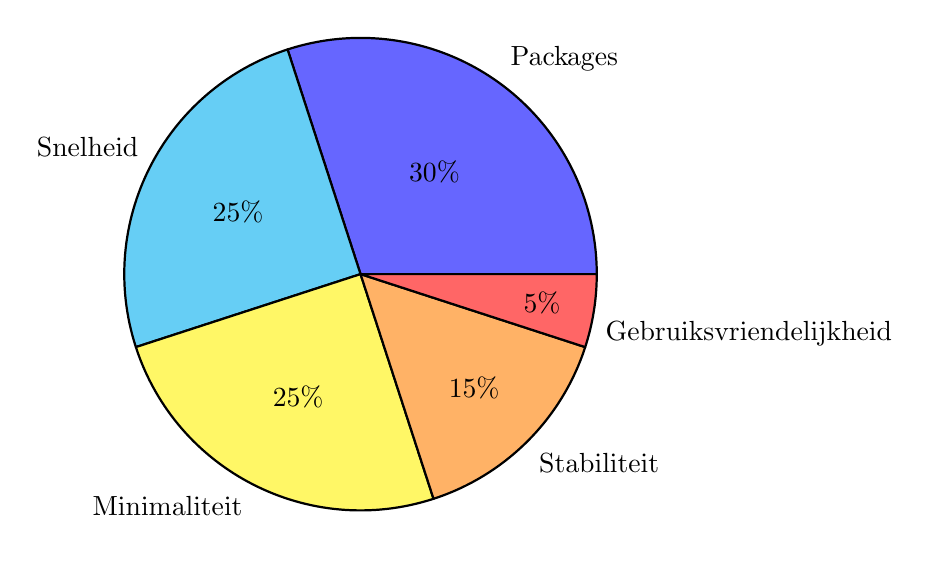
\begin{tikzpicture}

  \pie{30/Packages,
  25/Snelheid,
  25/Minimaliteit,
  15/Stabiliteit,
  5/Gebruiksvriendelijkheid}
  
\end{tikzpicture}
\caption{Belang van criteria}
\label{graph:spec_percentages}
\end{figure}

Zoals te zien in bovenstaand diagram, vind ik zelf packages het belangrijkst. 
Wat ik hiermee bedoel is de toegang tot programma's en daarbij ook nieuwe versies van programma's.
In Linux distributies worden programma's vooral gedownload vanaf package managers. Afhankelijk van de package manager kunnen programma's die hierop beschikbaar zijn behoorlijk achterlopen qua versie. 
\par\smallskip 
Met minimaliteit bedoel ik dat er weinig toegevoegd is aan het besturingssysteem. Dit heeft mijn persoonlijke voorkeur, omdat het hierdoor wat meer vrijheid biedt in de aanpasbaarheid en het over het algemeen wat sneller is. 
Ook gebruik ik op deze manier zo min mogelijk opslag, wat erg handig is in ons project.
\par\smallskip
Op basis van bovenstaande criteria ga ik de volgende distributies vergelijken. 
\begin{enumerate}
  \item Arch Linux, omdat ik deze distributie al gebruik en deze snel en erg minimalistisch is. 
  \item Ubuntu, omdat deze gebruikt werd door het vorige team en wordt gebruikt door het team van SailfishOS~\cite{sailfishportingguide}.
  \item Debian, omdat ubuntu hier op gebaseerd is en deze minimalistischer is dan Ubuntu. 
  \item Manjaro, omdat dit een gebruiksvriendelijke distributie is gebaseerd op Arch Linux 
\end{enumerate}

In de volgende tabel vergelijk ik de criteria. Op basis van deze criteria maak ik een toegelichte keuze\footnote{De scores in deze tabel zijn gebaseerd op subjectieve en anekdotische ervaringen, en algemene consensus binnen de Linux-gemeenschap. Zo is het, bijvoorbeeld, algemeen geaccepteerd in de Linux-gemeenschap dat een basisinstallatie van Arch Linux minimalistischer is dan een standaard Ubuntu-installatie.}.


\begin{table}[h]
  \centering
  \begin{tabular}{|l|c|c|c|c|c|}
    \hline
    \textbf{Besturingssysteem} & \textbf{Snelheid} & \textbf{Packages} & \textbf{Gebruiksgemak} & \textbf{Stabiliteit} & \textbf{Minimaliteit} \\
    \hline
    Arch Linux & ++ & ++ & - & + & ++ \\
    \hline
    Ubuntu & + & - & ++ & ++ & - \\
    \hline
    Debian & ++ & - & + & + & + \\
    \hline
    Manjaro & + & ++ & ++ & ++ & + \\
    \hline
  \end{tabular}
  \caption{Criteria score per distributie}
  \label{tab:os_ratings}
\end{table}

In bovenstaande tabel is te zien dat de keuze toch ligt tussen Arch Linux en Manjaro.
Hiertussen is Arch Linux wat minimalistischer, maar is Manjaro normaal gesproken wat stabieler en gebruiksvriendelijker. 
\par\smallskip
Op basis van deze punten kies ik voor Arch Linux. 
Arch Linux biedt toegang tot de AUR. Dit is een package repository die wordt onderhouden door de Arch Linux community.
Dit stelt een breed scala aan packages tot mijn beschikking, waarvan vele direct worden gebouwd vanuit Github.
Hiermee heb ik toegang tot bijna elk programma dat beschikbaar is op Linux, met daarbij de laatste versie. 
Daarnaast is Arch Linux snel en erg stabiel wanneer er wordt gekozen voor de LTS kernel. 
\par\smallskip
Hoewel het verschil tussen Manjaro en Arch Linux erg klein is, heb ik meer ervaring met Arch Linux en kan deze beter aangepast worden naar mijn wensen. 
Dit zal me beter in staat stellen om efficient te werken gedurende het project.


\personalchoice{Opzetten ontwikkelsysteem}
\subsubsection{Context}
\timestamp{2023-09-05}
Voor het opzetten van de ontwikkelomgeving moest er een keuze gemaakt worden op welke manier Linux geïnstalleerd wordt op de laptop. 
De opties waren als volgt.
\begin{enumerate}
  \item Linux in een Virtual Machine (VM)
  \item Dual booten naast Windows
  \item Native runnen, dat wil zeggen "direct op de laptop, zonder tussenlagen"
\end{enumerate}

Dual booten naast Windows is exact hetzelfde als native qua performance, omdat het direct op de hardware runt. 
Het enige verschil ten opzichten van native is dat je minder opslag hebt voor de Linux installatie. Dit komt omdat er natuurlijk ook ruimte nodig is voor Windows en de applicaties en documenten op Windows. 
\par\smallskip
Native is sneller dan virtual machines. Dit komt door de overhead die wordt toegevoegd door de Hypervisor. 
Hoeveel overhead dit is, hangt sterk af van veel factoren. Dit zijn dingen zoals de cpu, andere systeemonderdelen, de instellingen van de virtual machine, etc. 
Daarnaast is in de meeste gevallen een deel van de CPU, RAM en schijf nodig voor de host-besturingssysteem.
Maar, dat native sneller is dan virtual machine wordt aangetoond in een 2014 onderzoek van IBM~\cite{felter2015updated}.
Hierin wordt de performance van kernel-level virtual machines vergeleken met Docker en native. 
Hieruit komt dat native sneller is dan zowel Docker als (K)VM's. 

\subsubsection{Keuze}
\timestamp{2023-09-05}
Ik heb gekozen om het simpelweg native te runnen, omdat dit voor mij de meeste voordelen heeft.
Hoewel het snelheidsverschil tussen een VM en native niet verschrikkelijk is, voegt een VM wel onnodige overhead toe. 
Ik had al een native Linux installatie, dus ik had geen reden om over te stappen op een VM. 
Daarnaast heb ik ook geen Windows nodig, dus is dual booten ook onnodig. 
\par\smallskip
Native geeft mij dus het meeste opslag en de beste performance. 


\teamchoice{Communicatie}
\subsubsection{Context}
\timestamp{2023-09-05}
Binnen ons projectgroep zullen we veel moeten communiceren. Afspraken moeten gemaakt worden, bestanden moeten gedeeld worden en soms moeten we simpelweg vragen kunnen stellen.
Normaal zal communicatie eenvoudig zijn als we met elkaar aan tafel zitten, maar er zullen zich ook situaties voordoen waar we niet fysiek kunnen communiceren.
In dit geval zijn er duidelijke afspraken nodig voor hoe we communiceren.
\par \smallskip 
We hebben in totaal drie digitale omgevingen nodig.
\begin{enumerate}
  \item Een communicatiekanaal voor contact met de opdrachtgever.
  \item Een communicatiekanaal voor intern teamcontact.
  \item Een gedeelde plek voor bestandsopslag.
\end{enumerate}

De keuze van communicatiekanalen is gemaakt aan de hand van de volgende lijst aan communicatieplatforms, welke is opgesteld aan de hand van een aantal redenen.
De overweging elke optie binnen de lijst staat genoteerd aan de rechterzijde van tabel \ref{tab:comm_platforms}.
\begin{table}[H]
  \centering
  \begin{tabular}{|l|p{10cm}|}
    \hline
    \textbf{Platform} & \textbf{Overweging} \\
    \hline
    \href{https://discord.com/}{Discord} & Discord werd overwogen vanwege de mogelijkheden georganiseerde kanalen binnen een groep. Ook had onze opdrachtgever hier een sterke voorkeur voor. \\
    \hline
    \href{https://www.whatsapp.com/}{WhatsApp} & WhatsApp was een optie vanwege de voorkeuren binnen het team. \\
    \hline
    \href{https://www.microsoft.com/en-us/microsoft-teams/group-chat-software}{Microsoft Teams} & Microsoft Teams stond op de lijst vanwege de integraties met andere Microsoft producten, zoals Word, en de voorkeur van onze Gilde meester. \\
    \hline
    \href{https://slack.com/}{Slack} & Slack werd overwogen vanwege het gebruik van deze software binnen een ander project en het hierbij erg rijk was een opties en organisatie \\
    \hline
    \href{https://telegram.org/}{Telegram} & Telegram was een optie vanwege de populariteit en de mogelijkheid om bestanden te delen. \\
    \hline
  \end{tabular}
  \caption{Overwegingen voor Communicatieplatforms}
  \label{tab:comm_platforms}
\end{table}
Overige communicatieplatforms zijn niet overwogen door een gebrek aan bekendheid binnen het team, of doordat deze opties essentiële features achter een betaling verschuilde.
We hebben binnen het team immers geen beschikbaar budget voor dit soort applicaties.
\par\smallskip
Voor de bestandsopslag hebben we twee grote spelers, namelijk Google Drive en OneDrive. 
Beide zijn goede opties met vergelijkbare features. De reden dat we hebben gekozen om deze twee methodes te vergelijken is de populariteit van deze opties.
Doordat deze opties zo populair zijn, hadden onze teamleden hier al accounts op en waren we al bekwaam in het gebruik van deze services.

\subsubsection{Keuze}
\timestamp{2023-09-05}
Om onze keuze te maken, hebben we voor- en nadelen tegenover elkaar gezet voor elk platform in de volgende tabel.
\begin{table}[H]
  \centering
  \begin{tabular}{|l|p{6cm}|p{6cm}|}
    \hline
    \textbf{Platform} & \textbf{Voordelen} & \textbf{Nadelen} \\
    \hline
    \href{https://discord.com/}{Discord} & Georganiseerde kanalen, hoge aanpasbaarheid, opdrachtgever gebruikt het al, bekendheid binnen het team. & Minder organisatie features dan alternatieven. \\
    \hline
    \href{https://www.whatsapp.com/}{WhatsApp} & Snel en eenvoudig, geen nieuwe installaties nodig binnen team. Sterke teamvoorkeur. & Beperkte bestandsgrootte voor delen, afhankelijk van telefoonnummer. Weinig organisatie-tools. \\
    \hline
    \href{https://www.microsoft.com/en-us/microsoft-teams/group-chat-software}{Microsoft Teams} & Goede integratie met Microsoft-producten, ondersteund door de Hogeschool. & Werkt niet goed op bepaalde Linux distributies. Niet open-source. Betaalde functies. \\
    \hline
    \href{https://slack.com/}{Slack} & Rijk aan functies, goede organisatie van kanalen, integraties met andere tools. & Betaalde functies voor volledige toegang, kan ingewikkeld zijn om op te zetten. \\
    \hline
    \href{https://telegram.org/}{Telegram} & Snel, mogelijkheid om grote bestanden te delen, cloud-gebaseerde opslag. & Minder populair in zakelijke context, weinig bekendheid binnen team \\
    \hline
  \end{tabular}
  \caption{Voordelen en Nadelen van Communicatieplatforms}
  \label{tab:comm_pros_cons}
\end{table}

Op basis van bovenstaande voor- en nadelen hebben we als team de volgende keuzes gemaakt als communicatiemiddelen.
\par\smallskip
Om contact te houden met de opdrachtgever hebben we gekozen voor een Discord server.
We hebben hiervoor gekozen, omdat de opdrachtgever Discord gebruikt en elk teamlid hier al actief gebruik van maakte.
\par \smallskip 
Voor intern teamcontact gebruiken we een Whatsapp groep. Dit vond het team unaniem de beste optie. Hiermee kunnen we snel met elkaar in contact komen en hoeven we geen nieuwe apps te installeren. 
\par \smallskip
Voor bestandsopslag gebruiken we OneDrive. Vanuit de Hogeschool Utrecht krijgen we allemaal standaard een OneDrive omgeving.
Hier hebben we meer dan voldoende opslag voor bestanden. OneDrive integreert ook gemakkelijk met Microsoft Word. 
Dat was voor ons reden genoeg om te kiezen voor OneDrive boven Google Drive.


% \teamchoice{Programmeertaal}
% \subsubsection{Context}
% \timestamp{2023-09-05}
% Gedurende het project zullen we veel moeten programmeren. Hiervoor is een breed scala aan mogelijkheden.

% \subsubsection{Keuze}
% \timestamp{2023-09-05}
% De taal waarin geprogrammeerd gaat worden zal voornamelijk C/C++ zijn. Met een gedeelte bash bij de opstartscripts van Sailfish OS.  
% Deze keuze is gemaakt door de oorspronkelijke ontwikkelaars van SailfishOS, LineageOS en de ontwikkelgroep van afgelopen jaar.
% Wij hebben besloten deze keuze aan te houden, omdat er geen goed concreet voordeel is om de programmeertaal te veranderen. Daarnaast zou dit problemen veroorzaken en veel tijd kosten.


\teamchoice{Docker}
\subsubsection{Context}
\timestamp{20-09-2023}
De huidige build environment wordt opgezet aan de hand van een installation guide~\cite{fairphonegithub}.
Daarnaast is er een installatiescript aanwezig.
Deze zouden moeten werken, maar hebben we dit tot nu toe nergens gemakkelijk werkend gekregen.
Tijdens het debuggen gaat het steeds fout op verschillende punten. 
We vermoeden dat dit komt door overblijvende build files die naar allemaal onbekende plekken in ons systeem worden geschreven, gebaseerd op eerdere ervaringen in eerdere projecten.

\subsubsection{Keuze}
\timestamp{20-09-2023}
Met oog op overdraagbaarheid denken wij als team dat het een goede keuze is om een Docker environment op te gaan zetten. 
Hiermee zou de build environment eenvoudig overdraagbaar zijn en zou het gemakkelijk werken op in principe elk systeem, zonder dat er build files overblijven na een compilatie.
Dit zou ook tijd kunnen gaan schelen tijdens het debuggen~\cite{AffinityBridgeDockerProsCons}. 
\par\smallskip
Deze keuze staat tegenover een keuze gemaakt door een voorgaand ontwikkelingsteam binnen het Fairphone project. 
Dit team koos er voor om niet verder te gaan met Docker, omdat dit vrij lastig bleek en er tegen problemen werd gelopen.
Wij geloven dat het waardevol is om toch hiermee verder te gaan, omdat dit de overdraagbaarheid enorm vergroot. Wij denken dat deze problemen niet onoverkomelijk zijn.
Hoewel het ons nu meer tijd zal kosten om dit op te zetten, zal dit een potentieel toekomstig ontwikkelingsteam enorm veel tijd schelen.
Voor het opzetten schatte wij als team tijdens scrum poker zo een 20 manuren voor de opzet van Docker. Hoewel dat waarschijnlijk meer is dan het zou kosten om de build environment nu op te lossen, schatten wij dat de build environment meer problemen zal veroorzaken op een later stadium. 
Zo is het vorige team daar meerdere sprints mee bezig geweest en leek het steeds op andere punten fout te gaan.

\par\smallskip
De laatste reden voor het opzetten van de Docker omgeving, is omdat de opdrachtgever hier een sterke voorkeur voor had. Door het opzetten van een Docker omgeving, zal een toekomstig team geen weken meer bezig zijn om de build environment op te zetten. In plaats daarvan zal het minder dan een dagdeel moeten duren, namelijk het installeren van Docker en het runnen van de container.

\chapter{Bibliografie}
% \textit{Nog te doen...}
% \nocite{*} % This includes all entries from the .bib file, even if they're not cited in the document
\begingroup
\renewcommand{\chapter}[2]{} % Removes the 'Chapter' heading
\renewcommand{\addcontentsline}[3]{} % Prevents adding this specific entry to TOC
\bibliographystyle{ieeetr}
\bibliography{bronnen}
\endgroup

% \chapter{Bijlagen}
% \textit{Ruimte voor peer reviews}

\end{document}